\newpage
\subsection{Caso d'uso UC11 - Menù profilo utente}
\label{UC11}

\begin{figure}[ht]
	\centering
	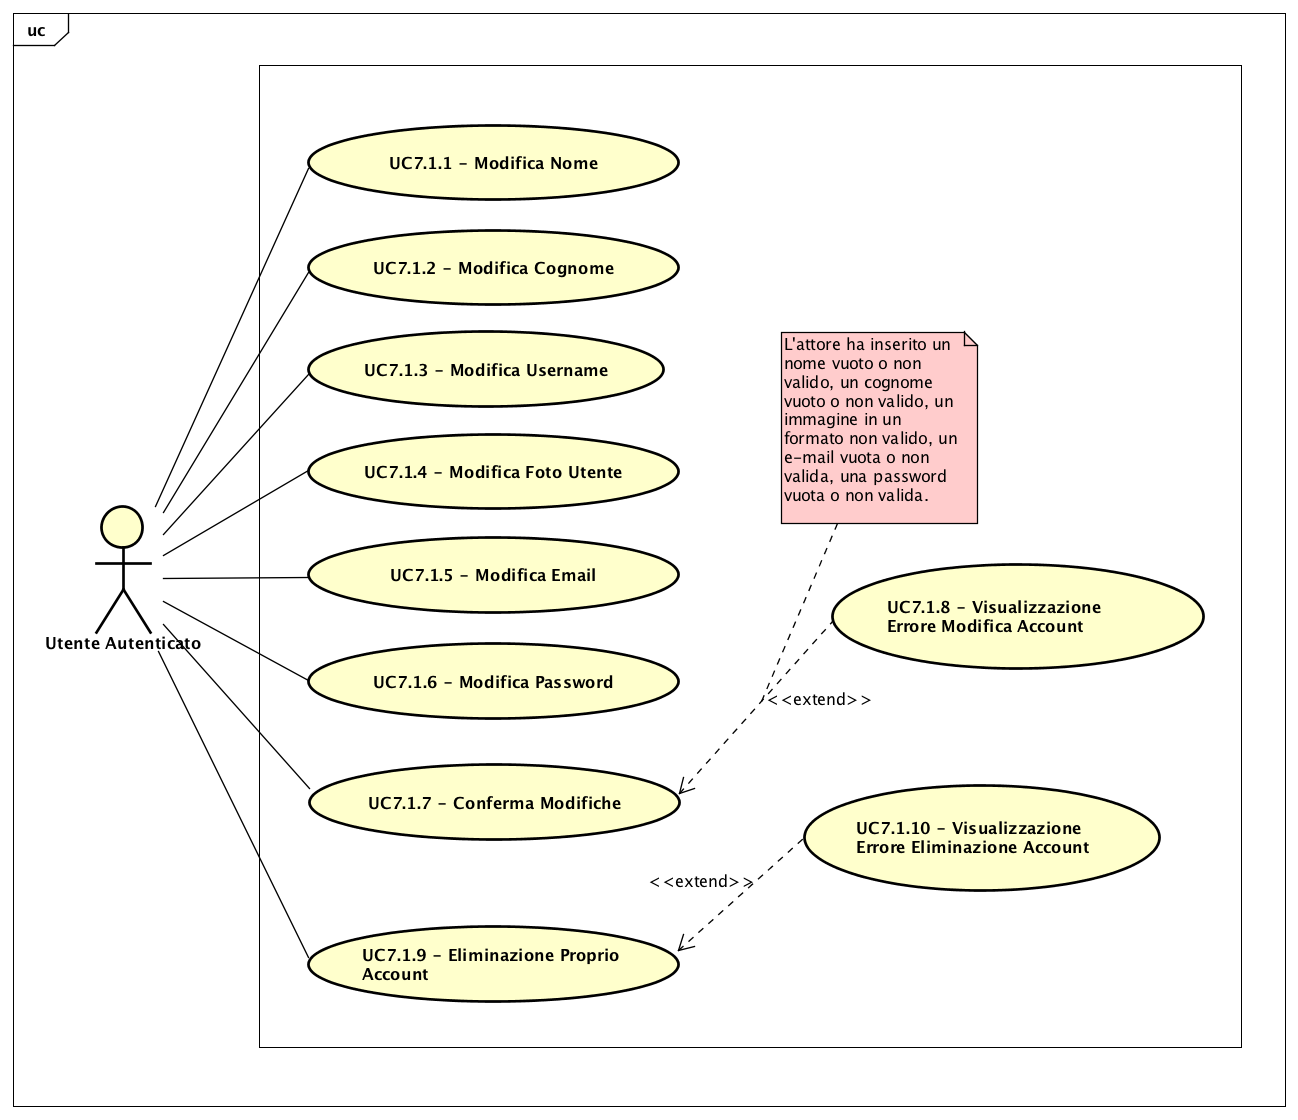
\includegraphics[scale=0.45]{UML/UC7_1.png}
	\caption{UC11 - Menù profilo utente}
\end{figure}
\FloatBarrier
\begin{longtable}{ l | p{11cm}}
	\hline
	\rowcolor{Gray}
	 \multicolumn{2}{c}{UC11 - Menù profilo utente} \\
	 \hline
	 \textbf{Attori} & Utente autenticato  \\
	\textbf{Descrizione} & L’attore può visualizzare e modificare i dati relativi all'account registrato \\
	\textbf{Pre-Condizioni} & L’attore è nel menù per la gestione del profilo \\
	\textbf{Post-Condizioni} & L’attore ha effettuato operazioni di gestione del proprio profilo \\
	\textbf{Scenario Principale} & 
	\begin{enumerate*}[label=(\arabic*.),itemjoin={\newline}]
		\item L'attore può gestire le proprie informazioni personali (UC11.1)
		\item L'attore può gestire il metodo di pagamento (UC11.2)
		\item L'attore può visualizzare le API acquistate (UC8)
		\item L'attore può interagire con le API da lui registrate e fornite sul marketplace (UCxx)
	\end{enumerate*}\\
\end{longtable}

\subsubsection{Caso d'uso UC11.1: Gestione informazioni personali}
\label{UC11_1}

\begin{minipage}{\linewidth}
	\begin{tabular}{ l | p{11cm}}
		\hline
		\rowcolor{Gray}
		\multicolumn{2}{c}{UC11.1 - Gestione informazioni personali} \\
		\hline
		\textbf{Attori} & Utente autenticato \\
		\textbf{Descrizione} & L'attore può gestire le proprie informazioni personali\\
		\textbf{Pre-Condizioni} & L'attore si trova nel menù relativo alla gestione delle informazioni personali del profilo\\
		\textbf{Post-Condizioni} & L'attore ha effettuato operazioni di gestione di informazioni personali \\
		\textbf{Scenario Principale} & 
		\begin{enumerate*}[label=(\arabic*.),itemjoin={\newline}]
			\item L'attore può visualizzare le informazioni personali (UC11.1.1)
			\item L'attore può modificare le informazioni personali (UC11.1.2)
		\end{enumerate*}
	\end{tabular}
\end{minipage}

\paragraph{Caso d'uso UC11.1.1: Visualizzazione info personali profilo utente}
\label{UC11_1_1}
\begin{figure}[ht]
	\centering
	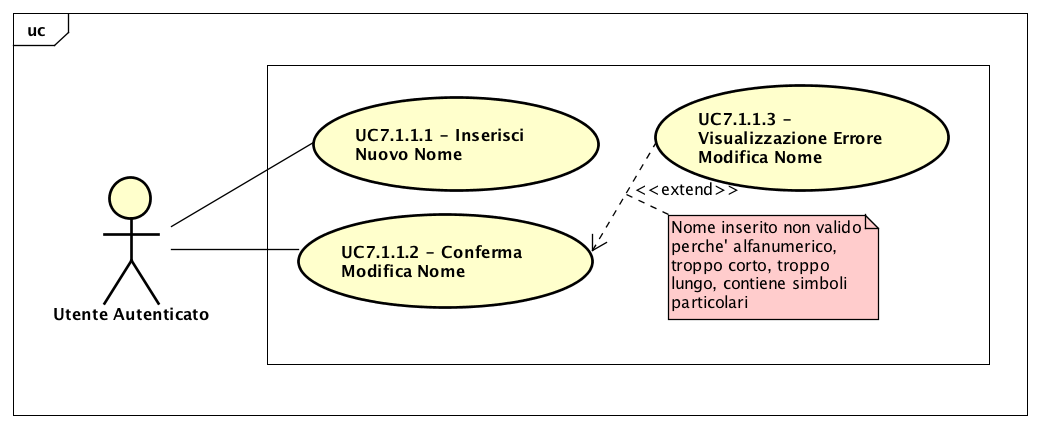
\includegraphics[scale=0.45]{UML/UC7_1_1.png}
	\caption{UC11.1.1: Visualizzazione info personali profilo utente}
\end{figure}
\FloatBarrier
\begin{tabular}{ l | p{11cm}}
	\hline
	\rowcolor{Gray}
	\multicolumn{2}{c}{UC11.1.1 - Visualizzazione info personali profilo utente} \\
	\hline
	\textbf{Attori} & Utente autenticato \\
	\textbf{Descrizione} & L'attore può visualizzare le informazioni personali relative al proprio account registrato\\
	\textbf{Pre-Condizioni} & L'attore è nella schermata di gestione informazioni personali\\
	\textbf{Post-Condizioni} & L'attore ha visualizzato le proprie informazioni personali \\
	\textbf{Scenario Principale} & 
	\begin{enumerate*}[label=(\arabic*.),itemjoin={\newline}]
		\item L'attore visualizza il nome (UC11.1.1.1)
		\item L'attore visualizza il cognome (UC11.1.1.2)
		\item L'attore visualizza lo username (UC11.1.1.3)
		\item L'attore visualizza l'email (UC11.1.1.4)
		\item L'attore visualizza l'immagine del profilo (UC11.1.1.5)
	\end{enumerate*}
\end{tabular}

\subparagraph{Caso d'uso UC11.1.1.1: Visualizzazione nome}
\label{UC11_1_1_1}
\begin{minipage}{\linewidth}
\begin{tabular}{ l | p{11cm}}
	\hline
	\rowcolor{Gray}
	\multicolumn{2}{c}{UC11.1.1.1 - Visualizzazione nome} \\
	\hline
	\textbf{Attori} & Utente autenticato \\
	\textbf{Descrizione} & L'attore può visualizzare il nome\\
	\textbf{Pre-Condizioni} & L'attore è nella schermata di visualizzazione informazioni personali\\
	\textbf{Post-Condizioni} & L'attore ha visualizzato il proprio nome \\
	\textbf{Scenario Principale} & 
	\begin{enumerate*}[label=(\arabic*.),itemjoin={\newline}]
		\item L'attore visualizza il proprio nome
	\end{enumerate*}
\end{tabular}
\end{minipage}

\subparagraph{Caso d'uso UC11.1.1.2: Visualizzazione cognome}
\label{UC11_1_1_2}
\begin{minipage}{\linewidth}
	\begin{tabular}{ l | p{11cm}}
		\hline
		\rowcolor{Gray}
		\multicolumn{2}{c}{UC11.1.1.2 - Visualizzazione cognome} \\
		\hline
		\textbf{Attori} & Utente autenticato \\
		\textbf{Descrizione} & L'attore può visualizzare il cognome\\
		\textbf{Pre-Condizioni} & L'attore è nella schermata di visualizzazione informazioni personali\\
		\textbf{Post-Condizioni} & L'attore ha visualizzato il proprio cognome \\
		\textbf{Scenario Principale} & 
		\begin{enumerate*}[label=(\arabic*.),itemjoin={\newline}]
			\item L'attore visualizza il proprio cognome
		\end{enumerate*}
	\end{tabular}
\end{minipage}

\subparagraph{Caso d'uso UC11.1.1.3: Visualizzazione username}
\label{UC11_1_1_3}
\begin{minipage}{\linewidth}
	\begin{tabular}{ l | p{11cm}}
		\hline
		\rowcolor{Gray}
		\multicolumn{2}{c}{UC11.1.1.3 - Visualizzazione username} \\
		\hline
		\textbf{Attori} & Utente autenticato \\
		\textbf{Descrizione} & L'attore può visualizzare lo username\\
		\textbf{Pre-Condizioni} & L'attore è nella schermata di visualizzazione informazioni personali\\
		\textbf{Post-Condizioni} & L'attore ha visualizzato il proprio username \\
		\textbf{Scenario Principale} & 
		\begin{enumerate*}[label=(\arabic*.),itemjoin={\newline}]
			\item L'attore visualizza il proprio username
		\end{enumerate*}
	\end{tabular}
\end{minipage}

\subparagraph{Caso d'uso UC11.1.1.4: Visualizzazione email}
\label{UC11_1_1_4}
\begin{minipage}{\linewidth}
	\begin{tabular}{ l | p{11cm}}
		\hline
		\rowcolor{Gray}
		\multicolumn{2}{c}{UC11.1.1.4 - Visualizzazione email} \\
		\hline
		\textbf{Attori} & Utente autenticato \\
		\textbf{Descrizione} & L'attore può visualizzare l'indirizzo email associato al proprio account\\
		\textbf{Pre-Condizioni} & L'attore è nella schermata di visualizzazione informazioni personali\\
		\textbf{Post-Condizioni} & L'attore ha visualizzato la propria email \\
		\textbf{Scenario Principale} & 
		\begin{enumerate*}[label=(\arabic*.),itemjoin={\newline}]
			\item L'attore visualizza la propria email
		\end{enumerate*}
	\end{tabular}
\end{minipage}

\subparagraph{Caso d'uso UC11.1.1.5: Visualizzazione immagine del profilo}
\label{UC11_1_1_5}
\begin{minipage}{\linewidth}
	\begin{tabular}{ l | p{11cm}}
		\hline
		\rowcolor{Gray}
		\multicolumn{2}{c}{UC11.1.1.5 - Visualizzazione immagine del profilo} \\
		\hline
		\textbf{Attori} & Utente autenticato \\
		\textbf{Descrizione} & L'attore può visualizzare l'immagine del profilo\\
		\textbf{Pre-Condizioni} & L'attore è nella schermata di visualizzazione informazioni personali\\
		\textbf{Post-Condizioni} & L'attore ha visualizzato l'immagine del proprio profilo \\
		\textbf{Scenario Principale} & 
		\begin{enumerate*}[label=(\arabic*.),itemjoin={\newline}]
			\item L'attore visualizza l'immagine del proprio profilo
		\end{enumerate*}
	\end{tabular}
\end{minipage}

\paragraph{Caso d'uso UC11.1.2: Modifica info personali profilo utente}
\label{UC11_1_2}
\begin{figure}[ht]
	\centering
	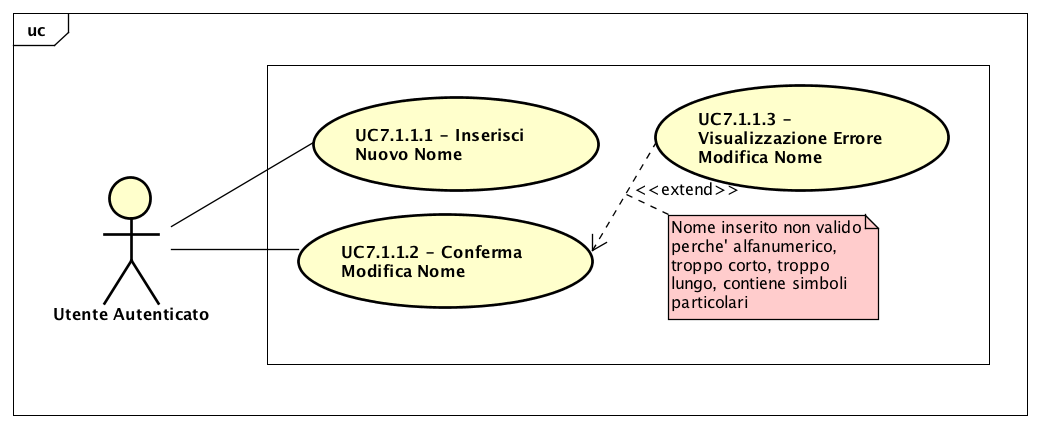
\includegraphics[scale=0.45]{UML/UC7_1_1.png}
	\caption{UC11.1.2: Modifica info personali profilo utente}
\end{figure}
\FloatBarrier
\begin{tabular}{ l | p{11cm}}
	\hline
	\rowcolor{Gray}
	\multicolumn{2}{c}{UC11.1.2 - Modifica info personali profilo utente} \\
	\hline
	\textbf{Attori} & Utente autenticato \\
	\textbf{Descrizione} & L'attore può modificare le informazioni personali relative al proprio profilo utente\\
	\textbf{Pre-Condizioni} & L'attore è nella schermata di gestione informazioni personali\\
	\textbf{Post-Condizioni} & L'attore ha modificato le proprie informazioni personali \\
	\textbf{Scenario Principale} & 
	\begin{enumerate*}[label=(\arabic*.),itemjoin={\newline}]
		\item L'attore può modificare il nome (UC11.1.2.1)
		\item L'attore può modificare il cognome (UC11.1.2.2)
		\item L'attore può modificare lo username (UC11.1.2.3)
		\item L'attore può modificare l'email (UC11.1.2.4)
		\item L'attore può modificare l'immagine del profilo (UC11.1.2.4)
		\item L'attore può confermare le modifiche effettuate (UC11.1.2.5)
	\end{enumerate*}\\
	\textbf{Scenari Alternativi} & 
	\begin{enumerate*}[label=(\arabic*.),itemjoin={\newline}]
		\item L'attore visualizza gli errori rilevati nelle modifiche richieste (UC)
	\end{enumerate*}\\
\end{tabular}

\subparagraph{Caso d'uso UC11.1.2.1: Modifica nome}
\label{UC11_1_2_1}
\begin{minipage}{\linewidth}
	\begin{tabular}{ l | p{11cm}}
		\hline
		\rowcolor{Gray}
		\multicolumn{2}{c}{UC11.1.2.1 - Modifica nome} \\
		\hline
		\textbf{Attori} & Utente autenticato \\
		\textbf{Descrizione} & L'attore può modificare il nome\\
		\textbf{Pre-Condizioni} & L'attore è nella schermata di modifica informazioni personali\\
		\textbf{Post-Condizioni} & L'attore ha modificato il nome \\
		\textbf{Scenario Principale} & 
		\begin{enumerate*}[label=(\arabic*.),itemjoin={\newline}]
			\item L'attore inserisce il nuovo nome
			\item L'attore conferma l'inserimento del nuovo nome
		\end{enumerate*}\\
		\textbf{Scenari Alternativi} & 
		\begin{enumerate*}[label=(\arabic*.),itemjoin={\newline}]
			\item L'attore visualizza un errore dovuto all'inserimento di un nome non consono
		\end{enumerate*}
	\end{tabular}
\end{minipage}

\subparagraph{Caso d'uso UC11.1.2.2: Modifica cognome}
\label{UC11_1_2_2}
\begin{minipage}{\linewidth}
	\begin{tabular}{ l | p{11cm}}
		\hline
		\rowcolor{Gray}
		\multicolumn{2}{c}{UC11.1.2.2 - Modifica cognome} \\
		\hline
		\textbf{Attori} & Utente autenticato \\
		\textbf{Descrizione} & L'attore può modificare il cognome\\
		\textbf{Pre-Condizioni} & L'attore è nella schermata di modifica informazioni personali\\
		\textbf{Post-Condizioni} & L'attore ha modificato il cognome \\
		\textbf{Scenario Principale} & 
		\begin{enumerate*}[label=(\arabic*.),itemjoin={\newline}]
			\item L'attore inserisce il nuovo cognome
			\item L'attore conferma l'inserimento del nuovo cognome
		\end{enumerate*}\\
		\textbf{Scenari Alternativi} & 
		\begin{enumerate*}[label=(\arabic*.),itemjoin={\newline}]
			\item L'attore visualizza un errore dovuto all'inserimento di un cognome non consono
		\end{enumerate*}
	\end{tabular}
\end{minipage}

\subsubsection{Caso d'uso UC11.2: Gestione metodo di pagamento}
\label{UC11_2}

\begin{minipage}{\linewidth}
	\begin{tabular}{ l | p{11cm}}
		\hline
		\rowcolor{Gray}
		\multicolumn{2}{c}{UC11.2 - Gestione metodo di pagamento} \\
		\hline
		\textbf{Attori} & Utente autenticato \\
		\textbf{Descrizione} & L'attore può gestire il proprio credito \\
		\textbf{Pre-Condizioni} & L'attore si trova nel menù relativo alla gestione del metodo di pagamento\\
		\textbf{Post-Condizioni} & L'attore ha effettuato operazioni relative al metodo di pagamento \\
		\textbf{Scenario Principale} & 
		\begin{enumerate*}[label=(\arabic*.),itemjoin={\newline}]
			\item L'attore può visualizzare il credito attuale presente nel proprio account (UC11.2.1)
			\item L'attore può effettuare un versamento per accrescere il proprio credito (UC11.2.2)
		\end{enumerate*}
	\end{tabular}
\end{minipage}

